\section{Feature Selection}
This phase serves a dual purpose. Firstly, since each type of feature (MFCC, Chroma, CQT, etc.) can consist of a varying number of individual features,
it is important to determine the optimal number of features for each type to maximize the model's performance.
Secondly, this phase aims to identify which specific features are the most relevant and influential for the classification task.
By doing so, we can enhance the model's efficiency and accuracy by focusing on the features that contribute the most to the classification process.

\subsection{Optimal number of features for each type of feature}
Considering that each type of feature can consist of a variable number of individual features,
it is necessary to determine the optimal number of features for each type to maximize the model's performance.
To achieve this, a `One Model per Feature' approach was employed. This involved training a separate model for each type of feature,
varying the number of features used. A set of 12, 20, 30, 40, 60, 70, 90, and 120 features was extracted for each type.Then, for each feature set,
three different models were trained using three classifiers: SVM, Random Forest, and Logistic Regression.\\
Figure \ref{fig:n_feature_per_type} shows the results obtained for each type of feature with the Random Forest model,
as it significantly outperformed the other classifiers.\\
The graph illustrates the F1 scores for different feature types, with varying numbers of features.
The MFCC features consistently achieved the highest F1 scores, peaking around 0.7.
This indicates that MFCC features are particularly effective for the classification task.
Interestingly, the number of features (from 30 to 120) does not drastically affect the performance, suggesting that even a smaller set of MFCC
features can be highly informative.\\
CQT features show moderate performance, with F1 scores around 0.4 to 0.5. The optimal number of features appears to be around 70,
beyond which there is no significant improvement. Similarly, RMS features exhibit a range of F1 scores from 0.4 to 0.5,
with optimal performance achieved with around 70 features.\\
For ZCR, SC, SB, and SR features, the F1 scores generally stabilize around 0.4 to 0.5.
Increasing the number of features beyond 40 does not result in significant performance gains and can even degrade the model's performance.
This suggests that adding too many features, especially those without strong predictive power, can confuse the model and degrade performance.\\
Overall, the optimal number of features is 30 MFCC,12 Chroma, 70 CQT, 40 RMS, 40 ZCR, 40 SC, 60 SB, and 40 SR.

\begin{figure*}[htbp]
    \centering
    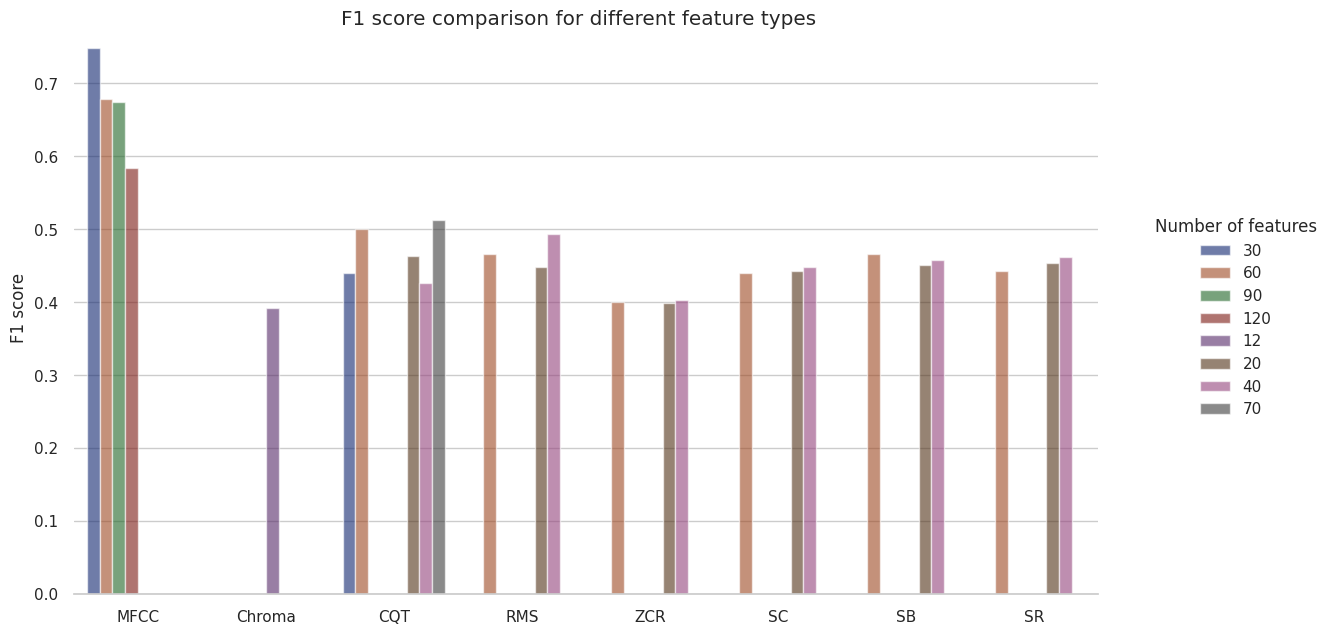
\includegraphics[width=.8\textwidth]{../images/n_feature_per_type.png}
    \caption{F1 score per number of features}
    \label{fig:n_feature_per_type}
\end{figure*}
\noindent
\subsection{Correlation analysis}
The previous analysis resulted in 338 features. Given this large number, it is necessary to perform an analysis to identify and remove features
that are poorly correlated with the target variable as well as those that are highly correlated with each other.
Due to the high number of features, a visual approach, such as a correlation matrix, was not feasible for identifying the features to be removed.
Instead, two filters were applied to select the most relevant features.\\
Since the normality test failed, the Spearman correlation coefficient was used for the analysis.\\
The first filter is based on the correlation between the features and the target variable. Features with a correlation below a certain
threshold with the target variable are removed. The second filter focuses on the correlation among the features themselves.
It counts, for each feature, the number of other features with which it has a correlation above a certain threshold. Features with a
number of correlations above a specified threshold are then removed.\\
The threshold values were chosen empirically. The filters were applied using the combinations of thresholds shown in Table \ref{tab:threshold_values}.

\rowcolors{2}{blue!8}{blue!18}
\begin{table}[h]
    \centering
    \small
    \begin{tabular}{|c|c|c|}
        \hline
        \textbf{Threshold} & \textbf{Values}                 \\
        THRESHOLD 1        & 0 - 0.1 - 0.2 - 0.3 - 0.4 - 0.5 \\
        THRESHOLD 2        & 0.6 - 0.7 - 0.8 - 0.9 - 1       \\
        N° FEATURES        & 5 - 10 - 15 - 20 - 25 - 30 - 40 \\
        \hline
    \end{tabular}
    \caption{threshold values}
    \label{tab:threshold_values}
\end{table}
\noindent
Using the filtered data, Random Forest models were trained to evaluate performance, as Random Forest was found to be the best performing model.
The combination of thresholds that led to the best performance was selected: threshold 1 = 0, threshold 2 = 0.6, and the number of features = 30.\\
From these results, it can be observed that with threshold 1 = 0, the filter on the correlation between the features and the target variable is effectively bypassed.
However, with threshold 2 = 0.6, a stringent filter is applied on the correlation among the features themselves, as all features with a correlation above 0.6
with at least 30 other features are removed. This indicates that it is more detrimental for the model to have features that are highly correlated
with each other than to have features that are poorly correlated with the target variable.\\
Figure \ref{fig:comparison_model_on_all_features_vs_model_on_best} shows the results obtained with the model trained on filtered features
compared to the model trained on all features. As can be seen, the model trained on filtered features performs significantly
better than the one trained on unfiltered features.

\begin{figure}[H]
    \centering
    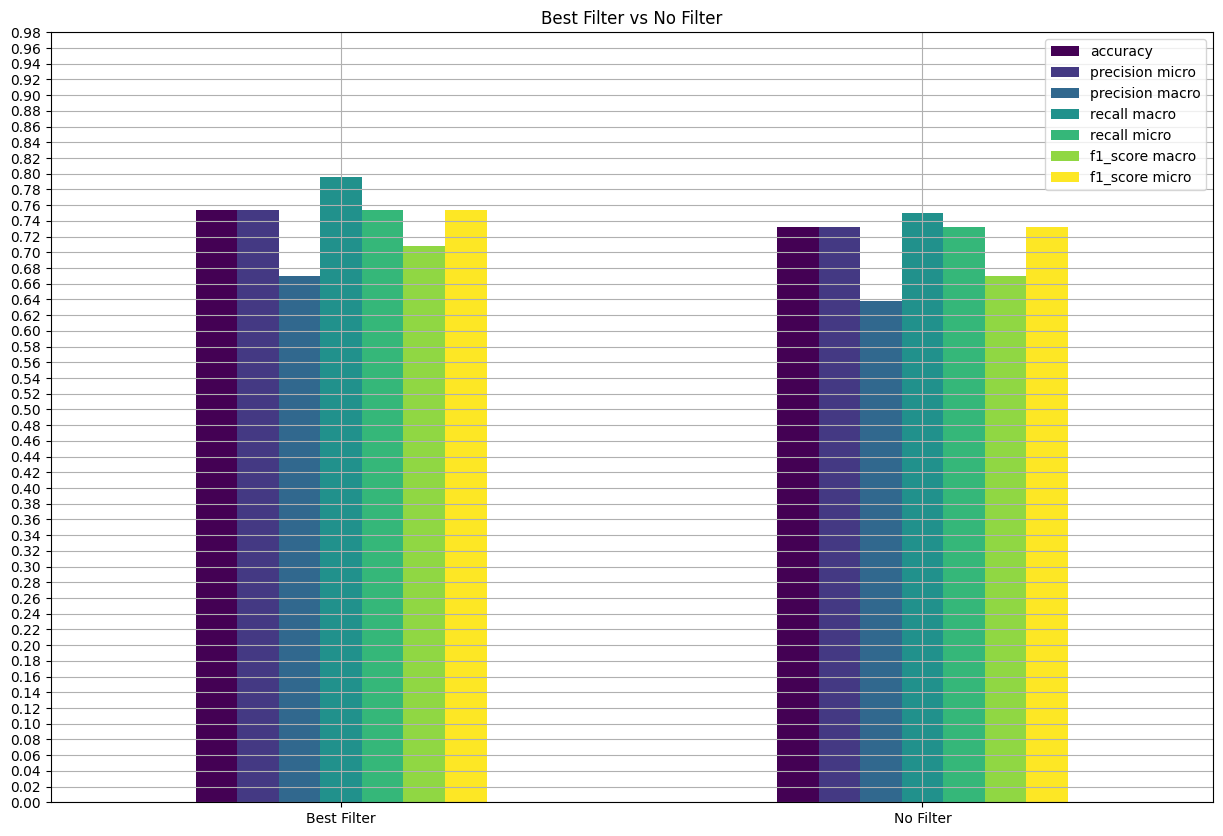
\includegraphics[width=0.8\columnwidth]{../images/model_on_all_features_vs_model_on_best.png}
    \caption{Comparison of different metrics between the model on all features and the model on the filtered ones}
    \label{fig:comparison_model_on_all_features_vs_model_on_best}
\end{figure}
\noindent
From the entire analysis, 41 features remained: 28 MFCC, 12 Chroma, and 1 ZCR.
The correlation matrix of the filtered features is shown in Figure \ref{fig:correlation_matrix}.
This matrix illustrates the pairwise correlation between the selected features, where the color intensity indicates the strength and direction of the correlation.
Dark red cells represent high positive correlations, while dark blue cells indicate high negative correlations.\\
The matrix demonstrates that the remaining features have low correlations with each other, as evidenced by the predominantly light colors away from the diagonal.
This implies that the features are relatively uncorrelated, which helps in preventing multicollinearity issues and enhances the robustness of the model.\\
The high diagonal values indicate that each feature is perfectly correlated with itself, which is expected.
However, the off-diagonal values being close to zero for most feature pairs confirm that the filtering process was effective in selecting
features that do not exhibit high inter-correlations. 

\begin{figure}[H]
    \centering
    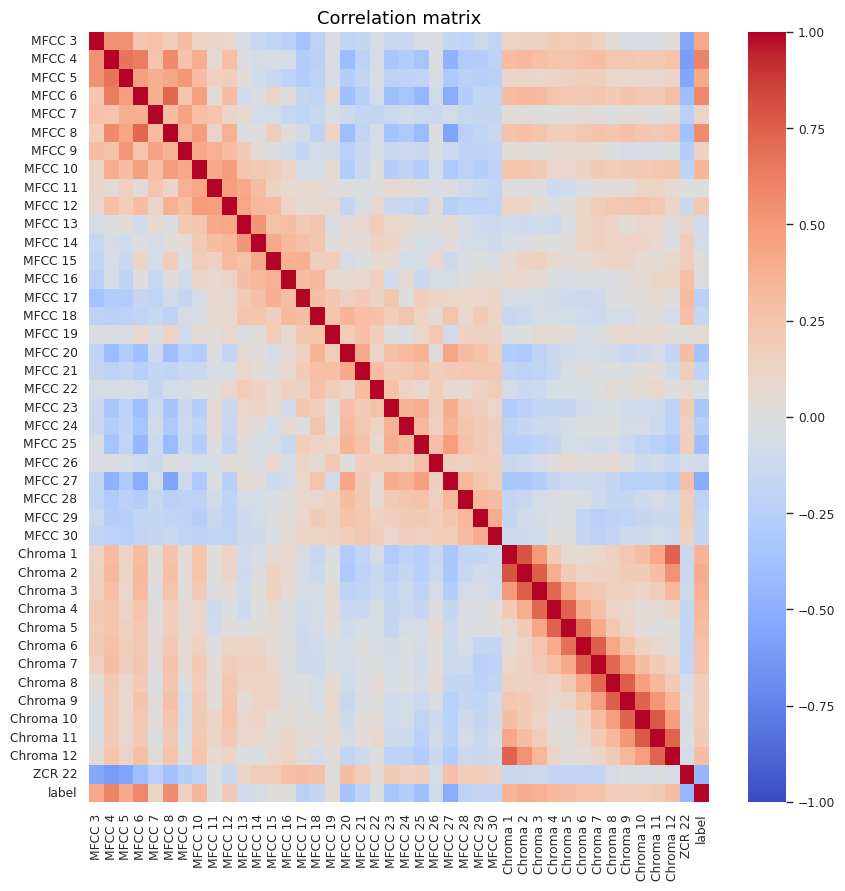
\includegraphics[width=0.8\columnwidth]{../images/correlation_matrix.png}
    \caption{Correlation matrix of the filtered features}
    \label{fig:correlation_matrix}
\end{figure}
